\documentclass[a4paper,10pt]{article}
\usepackage[margin=2.5cm]{geometry}
\usepackage[utf8]{inputenc}
\usepackage[T1]{fontenc}
\usepackage{lmodern}
\usepackage[colorlinks=true,urlcolor=blue,citecolor=blue]{hyperref}
\usepackage{amsmath,graphicx,float,caption,subcaption}
\usepackage{booktabs,tabularx,array}
\usepackage{tikz}
\usetikzlibrary{arrows.meta,positioning}
\setlength{\parindent}{0em}
\setlength{\parskip}{1em}
\setlength{\emergencystretch}{2em}
\clubpenalty=10000
\widowpenalty=10000
\brokenpenalty=10000
\captionsetup{font=small,labelfont=bf}
\title{\textbf{1RT730 Project Report}\\
EmployMee: A Source-Grounded Assistant\\for Swedish Tech Careers}
\author{Bradley Deku \and Elvia Dey \and Simran Khan}
\date{\today}
\begin{document}
	
\maketitle
    
 \section{Introduction}
 
Finding a job in Sweden can be challenging, especially for international students and people who have recently moved here. Job seekers often have to go through numerous advertisements, understand unfamiliar requirements, and figure out how to present their skills and experience. This becomes even more difficult when many advertisements are written in Swedish. Although large language models (LLMs) can explain technical skills and help with application writing, they do not always have access to current job listings or accurate information about what individual employers expect. They can also suggest CV changes that make a candidate’s experience sound stronger than it actually is.

To make this process easier, we developed \textbf{EmployMee}, an application that helps users explore technology jobs and master thesis opportunities in Sweden. Users can ask questions in their own words, browse original advertisements, upload their CVs, and compare their experience with the requirements listed by employers. They can also get suggestions for improving specific parts of their CV. The answers are provided in English, but users can still check the original advertisements in Swedish or English to see where the information comes from.

\textbf{EmployMee} uses retrieval-augmented generation (RAG), which allows the system to search relevant job advertisements before generating an answer \cite{rag}. It combines an automatically refreshed job database, hybrid multilingual search, metadata filters, and responses with citations. It also supports PDF text extraction and OCR when text cannot be extracted directly. For CV assistance, the system aims to distinguish between skills supported by the available evidence and requirements that cannot be verified from the CV. When the advertisements do not provide enough information, it is designed to acknowledge this rather than make unsupported claims. The goal is to help job seekers understand opportunities and present their existing experience more clearly, not to make hiring decisions on their behalf.

\section{Dataset}

\textbf{Source.}
EmployMee's knowledge base consists of publicly available job advertisements published by Arbetsf\"ormedlingen through the JobTech open data service \cite{jobtech}, which covers the advertisements listed on Platsbanken. The application downloads the current JobStream snapshot and keeps only the technical advertisements. Each advertisement is a text document with structured metadata: headline, employer, municipality, region, occupation, occupation field, publication date, application deadline, a link to the original advertisement, and the full description, available as plain text and as formatted HTML.

\textbf{Selection.}
We focus on technical roles and on thesis and degree project opportunities. An advertisement is kept if it belongs to the Data/IT occupation field, or if its headline or occupation label matches a list of English and Swedish technical role terms (for example software, cloud, cybersecurity, embedded, data engineer and \textit{systemutvecklare}). Because thesis advertisements often have generic titles, a thesis advertisement is also kept if its description mentions technical topics such as machine learning, programming or robotics. Thesis opportunities are identified by matching the headline and occupation label against English and Swedish thesis terms (e.g.\ ``thesis'', ``degree project'', \textit{examensarbete}, \textit{exjobb}). A thesis mentioned only in the requirements of an ordinary job does not count. These rules are keyword heuristics, so some relevant advertisements may be missed and some unrelated ones included.

\textbf{Snapshot used for evaluation.}
The snapshot used in our evaluation was recorded on 19 October 2026. It contains 3,472 advertisements, of which 25 are identified thesis opportunities, from 937 distinct employer names and 166 location entries. For retrieval, the advertisements were divided into 11,704 text chunks, about 3.4 per advertisement. These figures describe one point in time: advertisements are continuously added and removed, and the application refreshes its data automatically (Section~3).

\textbf{Preparation.}
Before indexing, we removed HTML markup, decoded character entities and normalized whitespace. Advertisements with an empty text, a duplicate advertisement ID, or identical cleaned text to an earlier advertisement were discarded. Missing metadata fields are filled with ``Not specified''. Advertisements are stored in their original language (mainly Swedish or English) and are not translated, which avoids translation errors and lets the multilingual embedding model work with the employer's own wording.

Each description is split into overlapping chunks of 320 tokens with an overlap of 60 tokens, measured with the tokenizer of the embedding model. Every chunk is prefixed with the advertisement's headline, employer, location and occupation, so that the embedding reflects which role the passage belongs to, and it carries the full metadata used for filtering and citations. Separately from the search chunks, the original formatting of each advertisement is read from the saved feed and sanitized (scripts, styles and images are removed, and obvious section labels are shown as headings) so that the user can inspect the advertisement as published next to the answer.

\textbf{Use of the data.}
The data serves only as a retrieval corpus; no model was trained or fine-tuned on it. The 15 retrieval test questions in Section~4 were generated from this snapshot with a fixed question template that names a role and employer, with one advertisement as the known correct answer for each. User CVs are never part of the dataset; they are handled per session only.

\textbf{Limitations and biases.}
The dataset does not represent the whole Swedish job market. It only contains advertisements available through JobTech that passed our filtering. Only exact duplicates are removed, so reposted advertisements with slightly different text remain, and missing metadata can weaken location and occupation filters for the affected advertisements. The quality of the advertisements depends on the employer: some state their requirements clearly, while others are vague or contain perks and generic recruitment text that adds noise to the chunks. The mix of Swedish and English wording may affect retrieval and interpretation. Finally, advertisements reflect the wording and assumptions of their authors, so biases in how requirements or ideal candidates are described can carry over into the system's answers.

\section{Architecture}

\begin{figure}[H]
\centering
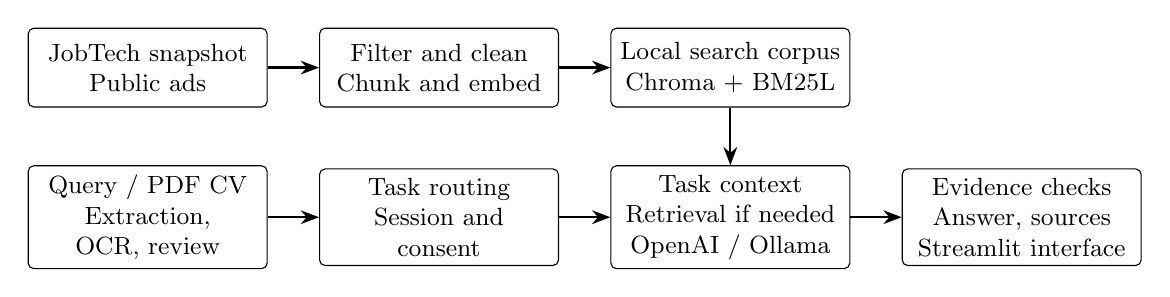
\begin{tikzpicture}[>=Stealth, every node/.style={font=\small},
 box/.style={draw,rounded corners=2pt,align=center,text width=2.8cm,minimum height=1.0cm},
 flow/.style={->,thick}]
\node[box] (feed) at (0,1.9) {JobTech snapshot\\Public ads};
\node[box] (prepare) at (3.7,1.9) {Filter and clean\\Chunk and embed};
\node[box] (store) at (7.4,1.9) {Local search corpus\\Chroma + BM25L};
\node[box] (input) at (0,0) {Query / PDF CV\\Extraction, OCR, review};
\node[box] (route) at (3.7,0) {Task routing\\Session and consent};
\node[box] (generate) at (7.4,0) {Task context\\Retrieval if needed\\OpenAI / Ollama};
\node[box] (output) at (11.1,0) {Evidence checks\\Answer, sources\\Streamlit interface};
\draw[flow] (feed) -- (prepare);
\draw[flow] (prepare) -- (store);
\draw[flow] (input) -- (route);
\draw[flow] (route) -- (generate);
\draw[flow] (store) -- (generate);
\draw[flow] (generate) -- (output);
\end{tikzpicture}
\caption{Main data flow. Retrieval is conditional on the task; general career advice and CV editing do not automatically become vacancy searches.}
\label{fig:architecture}
\end{figure}

\newpage
\textbf{Retrieval and freshness} 

The system uses a pretrained embedding model (\texttt{intfloat/multilingual-e5-small}) through Sentence Transformers\ \cite{e5}. Normalized embeddings are stored in a local Chroma collection using cosine distance. Long query/CV inputs are divided into 400-token segments and then their embeddings are averaged and normalized. This aggregation is a practical approximation and may dilute a specialized skill mentioned briefly in a CV.

Semantic retrieval is combined with lexical BM25L ranking. By default, six chunks are returned, with at most two per advertisement, to reduce repetition. Filters such as location, occupation and opportunity-type are used to narrow the candidates. The job data is refreshed when a page is loaded, if the last successful update is more than six hours old.

\textbf{Conversation and model integration} 

A rule-based router distinguishes job searches, questions about a specific advertisement, CV matching, tailoring, rewrites, career advice, greetings and follow-ups. This allows general questions to be answered without returning job ads every time. Prompting is used to avoid answering questions unrelated to jobs, companies, skills and other relevant topics. 

To maintain context about the user's skills, the CV is supplied on runs for as long as it remains enabled. This is also done to allow follow up questions to be asked. The smaller models often used job-posting times as current date/time so we override that at runtime by using the system clock, in our case, in Europe/Stockholm. 


The default model used OpenAI's  \texttt{gpt-6-luna} accessible via API calls. Given that this model is state-of-the art and well guarded, we implemented a local Ollama-based alternative. For this project, Alibaba's Qwen2.5 7B is run locally through Ollama. 


Task-specific instructions request English answers, distinguish general advice from employer facts, and treat advertisements and CVs as untrusted data rather than instructions. This reduces the risk of prompt injection, where text hidden in an advertisement or CV tries to override the system's rules.


\textbf{User Interface}

The underlying architecture is tied together by a user interface developed using Streamlit. It is divided into two sections. On the left is a control panel on the left that has features like model selection, CV uploading and review, and filtering. On the right side, the main chatbot interface, following the intuitive and commonly used opening/introductory prompt and textbar layout. Answers to general questions, such as job searches and advertisement questions, are streamed to the interface as they are generated. CV comparison, tailoring and rewriting answers are buffered and checked against the source text first, so they are displayed only once the final response is ready.


\textbf{CV processing and output checks} 

The application accepts PDF files with uploads limited to 10 MB and 12 pages or direct textbox entries up to 16,000 characters. Pages with insufficient text, or all pages when requested, are rendered and processed with local Tesseract OCR. English and Swedish language packs are supported. Users are able to review extraction errors in the control panel on the left of the user interface, before enabling model-provider consent. Once this is done, the reviewed text is sent to the selected generation provider. We do not save CVs to disk or embed them in the shared job index.

For CV comparisons, the model proposes structured ad statements and CV quotations. Matching/similar quotations from the retrieved ad and the CV are presented for the user to compare and see why the job is recommended. Unsupported quotations/recommendations are omitted or marked as lacking direct evidence. 


\section{Results}

We evaluated EmployMee through automated tests and a comparison of three retrieval methods. Our goal was to check that the application worked as expected and to understand how well different approaches to searching for jobs could find relevant advertisements.

\subsection{Application Testing}

We ran the project's automated test suite, which completed successfully with 194 passing tests in 4.62 seconds. These tests covered important parts of the application, including job searching, CV processing, conversation handling, citations, and the user interface.

During development, we also identified and addressed several issues. For example, some CV-related questions initially returned unrelated job advertisements, and follow-up questions sometimes lost track of the user's previous context. We made changes to how the application handles different types of questions and maintains conversation information to make the system more robust.

Although the automated tests passed, some relied on simulated model responses. Therefore, these results show that the tested functions behaved as expected, rather than proving that every response generated by the application will be accurate.

\subsection{Retrieval Performance}

To compare the retrieval methods, we created 15 test questions based on job advertisements present in our dataset. Each question asked about a specific position and employer, allowing us to check whether the correct advertisement appeared in the retrieved results.

We compared three approaches:
\begin{itemize}
    \item Keyword search, which matches words in the question with words in advertisements.
    \item Semantic search, which uses embeddings to find advertisements with similar meanings.
    \item Hybrid search, which combines both keyword and semantic retrieval.
\end{itemize}

All three methods were tested using the same questions and dataset of 3,472 advertisements, divided into 11,704 searchable chunks. We recorded how often the correct advertisement was retrieved, how highly it was ranked, and the time taken to retrieve results.

\begin{table}[htbp]
\centering
\begin{tabular}{lccc}
\toprule
Method & Correctly Retrieved & MRR & Median Time \\
\midrule
Keyword & 8/15 (53.3\%) & 0.367 & 617 ms \\
Semantic & 15/15 (100\%) & 1.000 & 15 ms \\
Hybrid & 15/15 (100\%) & 0.833 & 629 ms \\
\bottomrule
\end{tabular}
\caption{Comparison of retrieval methods across 15 test questions. MRR measures how highly the correct advertisement appears in the results, with higher values indicating better rankings.}
\label{tab:retrieval}
\end{table}

Semantic search performed best in this experiment. It retrieved the correct advertisement for all 15 questions and consistently ranked it first. Hybrid search also found all 15 advertisements, although the correct result was not always ranked first.

Keyword search performed less well, finding the correct advertisement in only 8 of the 15 questions. It was also slower than semantic search in our implementation.

One interesting finding was that combining keyword and semantic search did not improve the results compared with semantic search alone. This suggests that adding another retrieval method does not necessarily lead to better performance, particularly when the semantic model already identifies the relevant advertisement.

However, the questions used in this experiment included the exact job titles and employers. They were therefore easier to match than more general questions that users might ask, such as which skills are most commonly required for data science positions. The results should, therefore, be interpreted as an initial comparison rather than a complete measure of the system's retrieval accuracy.

\subsection{Observations and Limitations}

Overall, the testing showed that the main application components were functioning as expected and that semantic retrieval was particularly effective for finding specific job advertisements in our dataset.

While we did not conduct a separate user study, we also observed improvements in how the application handled CV questions, relevant follow-up conversations not directly related to the CV or jobs, and the presentation of original job advertisements as we addressed issues during development. These improvements were checked through development testing.

The main limitation of our evaluation is the small number of retrieval questions and their focus on finding known advertisements. We have not yet formally evaluated the accuracy of generated answers, compared the quality of responses from different language models, or measured how useful the application is to real job seekers. A more complete evaluation would include these as well as a larger set of independently reviewed questions in both Swedish and English.


\section{Societal Impact}

\subsection{Benefits}
Finding a job in Sweden can be difficult, particularly for international students who are still getting used to the language and job market. EmployMee makes the process easier by allowing users to explore job advertisements in English and understand what employers are looking for without spending hours searching through different websites. Since answers include citations, users can check the original advertisements and see where the information comes from. The searchable technical terms and PDF/OCR support also make it easier to understand job requirements, identify relevant projects, and explain how their existing skills relate to a position.

\subsection{Risks and Ethical Considerations}
Despite these benefits, the application has some limitations. It may misunderstand an advertisement or provide incorrect information, which could cause users to overlook a suitable position or misunderstand an employer’s requirements. Biases already present in job advertisements may also appear in the system’s answers. Additionally, users may trust an answer simply because it sounds convincing. The search and matching process may miss relevant jobs, especially when a candidate describes their experience differently from the wording used in an advertisement. Similarly, gaps in a CV, an unfamiliar educational background, or errors in extracting PDF text should not be taken as signs of a lack of ability. Since the system has not been tested for fairness across different languages and user groups, its recommendations should be used with care.

Privacy is another important concern because CVs often contain personal details. Although the application follows specific data-handling measures, external model providers such as OpenAI may have their own data-retention and logging practices. The system may also suggest CV changes that are inaccurate, respond incorrectly to misleading instructions hidden in input documents (prompt injection), or encourage users to rely too heavily on AI-generated advice. Finally, running language models, processing PDFs, and updating the job database all require computing resources. The application’s energy use and environmental impact have not been measured.

\subsection{Mitigation Strategies}
Several measures are used to reduce these risks. The application provides citations, bases answers on retrieved job advertisements, and acknowledges when the available information is insufficient. Users are encouraged to read the original advertisements before making decisions, and the system is intended to assist job seekers rather than make hiring decisions. It also separates missing evidence from a lack of ability, distinguishes required skills from preferred ones, and does not assume that Swedish proficiency is necessary just because an advertisement is written in Swedish.

For CV assistance, the application uses conservative rewriting, checks quoted text, and encourages users to review suggested changes before using them. These measures can reduce unsupported claims, but they cannot guarantee that every suggestion is correct. To protect privacy, PDF extraction and OCR take place locally in the current deployment. Reviewed text is sent to the selected model provider only after the user gives consent, and users are encouraged to remove personal details that are not needed. Consent is reset when the provider changes, and CVs and chat history are kept in session memory rather than deliberately saved by the application. However, disabling response storage does not necessarily prevent a provider from retaining other logs or records.

The application also reuses cached data, updates embeddings incrementally, uses local retrieval, answers clock questions without calling a model, and skips retrieval when a question does not need job ads, to avoid unnecessary computation. Overall, these measures help make the application more transparent and reduce potential harm while keeping users in control. However, they cannot remove every risk or guarantee that the system will always be accurate, fair, or environmentally sustainable.

\section*{Use of generative AI}
Generative AI assistance through Codex was used during implementation, debugging, interface/branding development and preparation of this report draft. Tests were also generated to assess the functioning of the application. 

\begin{thebibliography}{9}
\bibitem{rag} P. Lewis et al. \textit{Retrieval-Augmented Generation for Knowledge-Intensive NLP Tasks}. NeurIPS, 2020. \url{https://arxiv.org/abs/2005.11401}.

\bibitem{jobtech} Arbetsf\"ormedlingen. \textit{JobStream: Open Job Advertisement Data}. Accessed 19 October 2026. \url{https://data.jobtechdev.se/dataservice/data-service-jobstream/}.

\bibitem{e5} intfloat. \textit{multilingual-e5-small: Model Card}. Accessed 19 October 2026. \url{https://huggingface.co/intfloat/multilingual-e5-small}.

\end{thebibliography}
	
	
\pagebreak

\appendix
\section{GitHub Repository}

The complete source code, implementation details, and instructions for running the EmployMee application are available in our GitHub repository:

    \url{https://github.com/bradleybands/LLM-project-group-13}

Note that all commits are made by one github user account since the team decided to primarily work in-person and on one machine that could run the models locally.

\end{document}